\documentclass[12pt]{article}
\usepackage{graphicx}
\usepackage{float}
%\graphicspath{{Figures/}}		% path to graphic files
\usepackage{fullpage}


\begin{document}
	\begin{verbatim}
		fitted_curve = 
		
		General model:
		fitted_curve(x) = a*exp(b*x)+c
		Coefficients (with 95% confidence bounds):
		a =       41.07  (30.2, 51.94)
		b =   -0.001378  (-0.002099, -0.0006565)
		c =       28.06  (16.03, 40.08)
		
		gof = 
		
		struct with fields:
		
		sse: 2.2951e+02
		rsquare: 9.3155e-01
		dfe: 34
		adjrsquare: 9.2752e-01
		rmse: 2.5981e+00
	\end{verbatim}
	\begin{equation}
		\alpha=28.06+41.07\exp( -0.001378T); \quad T[K], \alpha [m^2/s]
	\end{equation}
	
	
	% \end{figure}

\begin{figure}[h!]
	\centering
	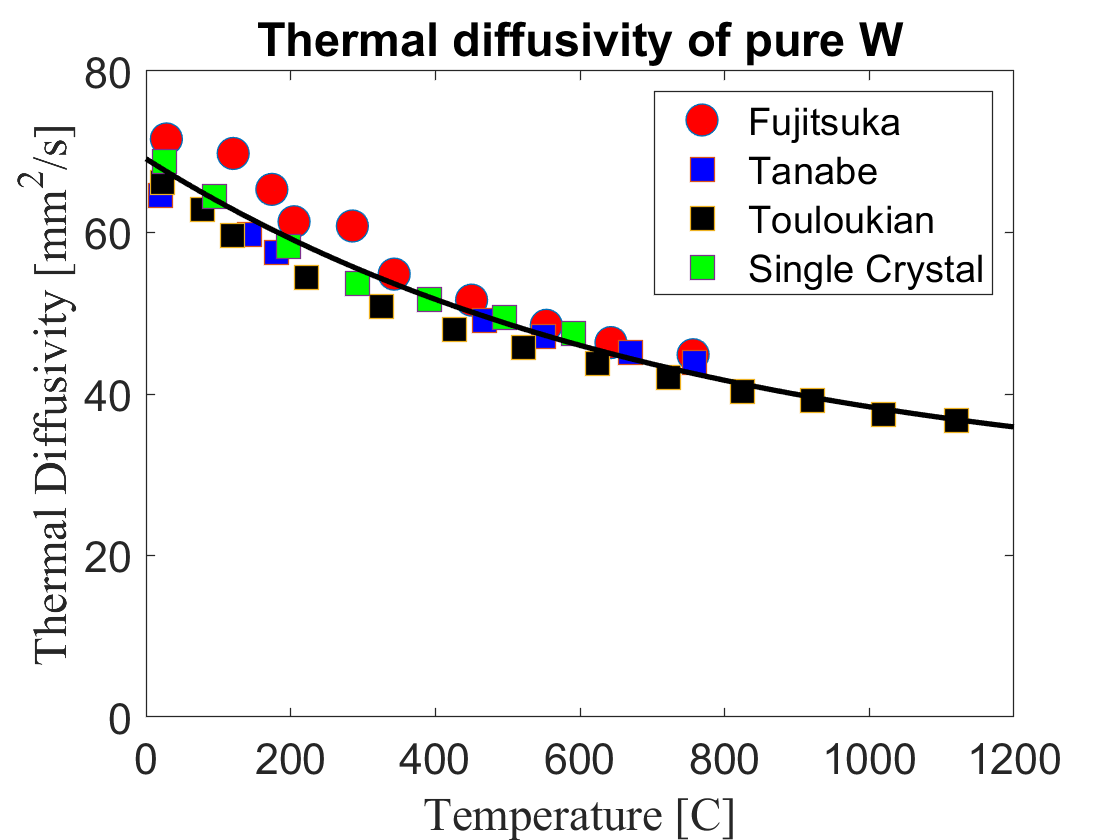
\includegraphics[width=0.75\linewidth]{W_diffusivity}  
	\caption{Tungsten thermal diffusivity.}
	\label{fig:W_fab1}
\end{figure}
\end{document}